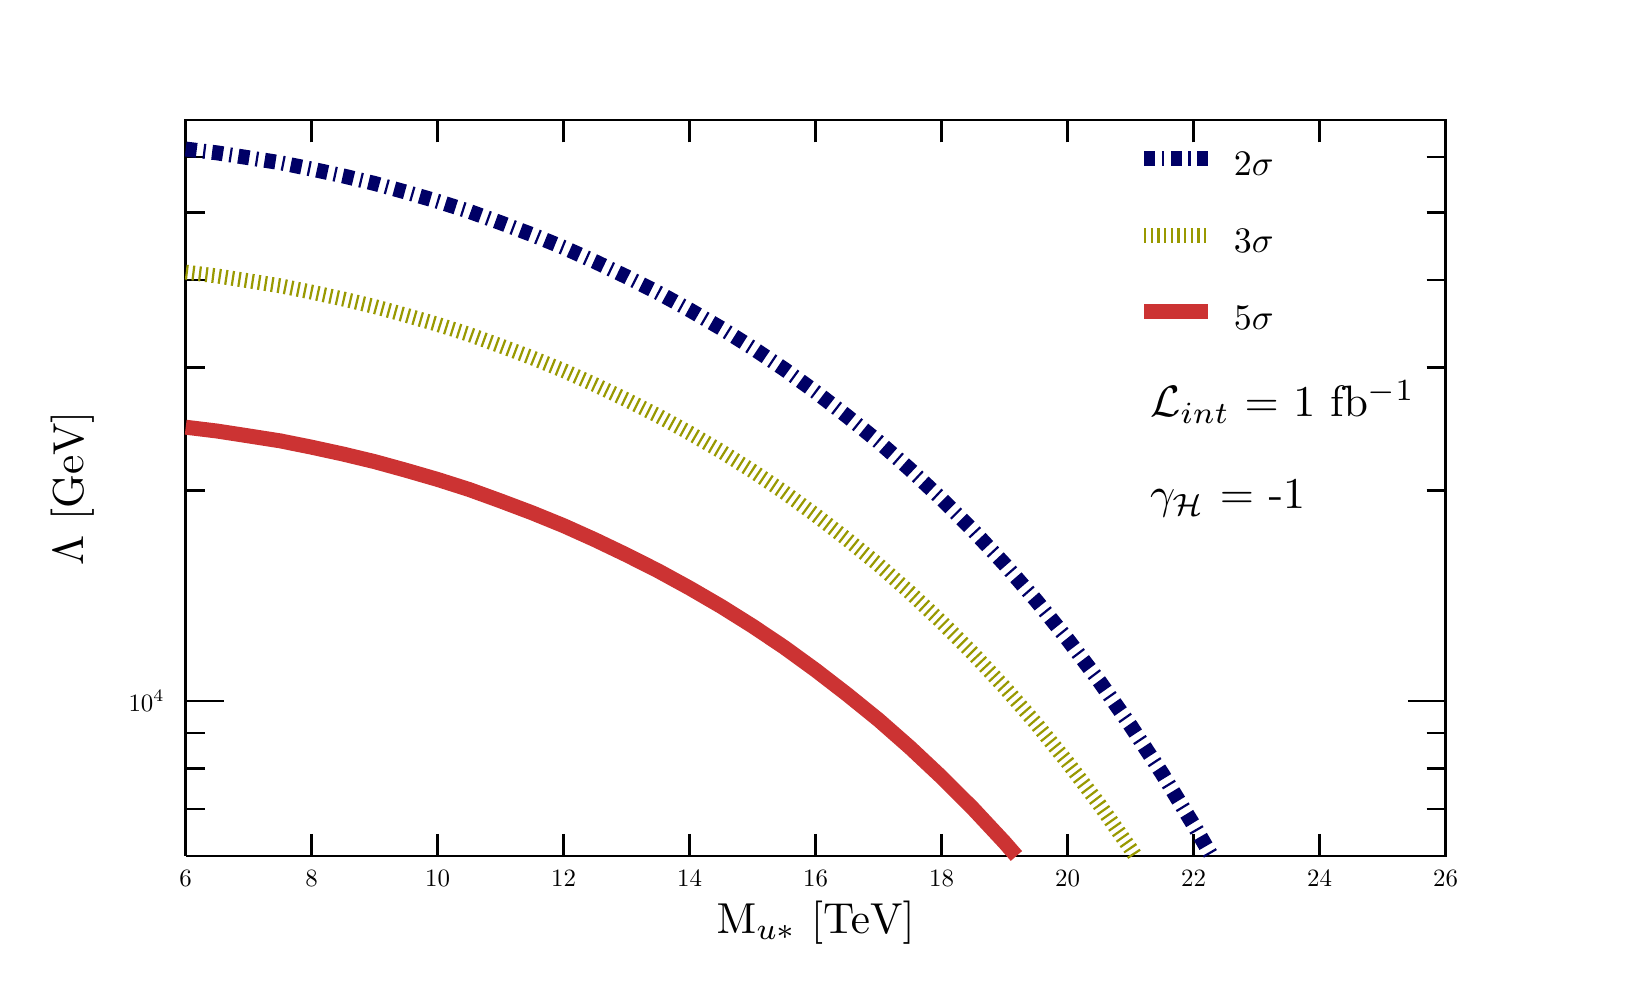
\begin{tikzpicture}
\pgfdeclareplotmark{cross} {
\pgfpathmoveto{\pgfpoint{-0.3\pgfplotmarksize}{\pgfplotmarksize}}
\pgfpathlineto{\pgfpoint{+0.3\pgfplotmarksize}{\pgfplotmarksize}}
\pgfpathlineto{\pgfpoint{+0.3\pgfplotmarksize}{0.3\pgfplotmarksize}}
\pgfpathlineto{\pgfpoint{+1\pgfplotmarksize}{0.3\pgfplotmarksize}}
\pgfpathlineto{\pgfpoint{+1\pgfplotmarksize}{-0.3\pgfplotmarksize}}
\pgfpathlineto{\pgfpoint{+0.3\pgfplotmarksize}{-0.3\pgfplotmarksize}}
\pgfpathlineto{\pgfpoint{+0.3\pgfplotmarksize}{-1.\pgfplotmarksize}}
\pgfpathlineto{\pgfpoint{-0.3\pgfplotmarksize}{-1.\pgfplotmarksize}}
\pgfpathlineto{\pgfpoint{-0.3\pgfplotmarksize}{-0.3\pgfplotmarksize}}
\pgfpathlineto{\pgfpoint{-1.\pgfplotmarksize}{-0.3\pgfplotmarksize}}
\pgfpathlineto{\pgfpoint{-1.\pgfplotmarksize}{0.3\pgfplotmarksize}}
\pgfpathlineto{\pgfpoint{-0.3\pgfplotmarksize}{0.3\pgfplotmarksize}}
\pgfpathclose
\pgfusepathqstroke
}
\pgfdeclareplotmark{cross*} {
\pgfpathmoveto{\pgfpoint{-0.3\pgfplotmarksize}{\pgfplotmarksize}}
\pgfpathlineto{\pgfpoint{+0.3\pgfplotmarksize}{\pgfplotmarksize}}
\pgfpathlineto{\pgfpoint{+0.3\pgfplotmarksize}{0.3\pgfplotmarksize}}
\pgfpathlineto{\pgfpoint{+1\pgfplotmarksize}{0.3\pgfplotmarksize}}
\pgfpathlineto{\pgfpoint{+1\pgfplotmarksize}{-0.3\pgfplotmarksize}}
\pgfpathlineto{\pgfpoint{+0.3\pgfplotmarksize}{-0.3\pgfplotmarksize}}
\pgfpathlineto{\pgfpoint{+0.3\pgfplotmarksize}{-1.\pgfplotmarksize}}
\pgfpathlineto{\pgfpoint{-0.3\pgfplotmarksize}{-1.\pgfplotmarksize}}
\pgfpathlineto{\pgfpoint{-0.3\pgfplotmarksize}{-0.3\pgfplotmarksize}}
\pgfpathlineto{\pgfpoint{-1.\pgfplotmarksize}{-0.3\pgfplotmarksize}}
\pgfpathlineto{\pgfpoint{-1.\pgfplotmarksize}{0.3\pgfplotmarksize}}
\pgfpathlineto{\pgfpoint{-0.3\pgfplotmarksize}{0.3\pgfplotmarksize}}
\pgfpathclose
\pgfusepathqfillstroke
}
\pgfdeclareplotmark{newstar} {
\pgfpathmoveto{\pgfqpoint{0pt}{\pgfplotmarksize}}
\pgfpathlineto{\pgfqpointpolar{44}{0.5\pgfplotmarksize}}
\pgfpathlineto{\pgfqpointpolar{18}{\pgfplotmarksize}}
\pgfpathlineto{\pgfqpointpolar{-20}{0.5\pgfplotmarksize}}
\pgfpathlineto{\pgfqpointpolar{-54}{\pgfplotmarksize}}
\pgfpathlineto{\pgfqpointpolar{-90}{0.5\pgfplotmarksize}}
\pgfpathlineto{\pgfqpointpolar{234}{\pgfplotmarksize}}
\pgfpathlineto{\pgfqpointpolar{198}{0.5\pgfplotmarksize}}
\pgfpathlineto{\pgfqpointpolar{162}{\pgfplotmarksize}}
\pgfpathlineto{\pgfqpointpolar{134}{0.5\pgfplotmarksize}}
\pgfpathclose
\pgfusepathqstroke
}
\pgfdeclareplotmark{newstar*} {
\pgfpathmoveto{\pgfqpoint{0pt}{\pgfplotmarksize}}
\pgfpathlineto{\pgfqpointpolar{44}{0.5\pgfplotmarksize}}
\pgfpathlineto{\pgfqpointpolar{18}{\pgfplotmarksize}}
\pgfpathlineto{\pgfqpointpolar{-20}{0.5\pgfplotmarksize}}
\pgfpathlineto{\pgfqpointpolar{-54}{\pgfplotmarksize}}
\pgfpathlineto{\pgfqpointpolar{-90}{0.5\pgfplotmarksize}}
\pgfpathlineto{\pgfqpointpolar{234}{\pgfplotmarksize}}
\pgfpathlineto{\pgfqpointpolar{198}{0.5\pgfplotmarksize}}
\pgfpathlineto{\pgfqpointpolar{162}{\pgfplotmarksize}}
\pgfpathlineto{\pgfqpointpolar{134}{0.5\pgfplotmarksize}}
\pgfpathclose
\pgfusepathqfillstroke
}
\definecolor{c}{rgb}{1,1,1};
\draw [color=c, fill=c] (0,0) rectangle (20,11.6806);
\draw [color=c, fill=c] (2,1.16806) rectangle (18,10.5125);
\definecolor{c}{rgb}{0,0,0};
\draw [c,line width=0.9] (2,1.16806) -- (2,10.5125) -- (18,10.5125) -- (18,1.16806) -- (2,1.16806);
\definecolor{c}{rgb}{1,1,1};
\draw [color=c, fill=c] (2,1.16806) rectangle (18,10.5125);
\definecolor{c}{rgb}{0,0,0};
\draw [c,line width=0.9] (2,1.16806) -- (2,10.5125) -- (18,10.5125) -- (18,1.16806) -- (2,1.16806);
\draw [c,line width=0.9] (2,1.16806) -- (18,1.16806);
\draw (10,0.327056) node[scale=1.56475, color=c, rotate=0]{M$_{u*}$ [TeV]};
\draw [c,line width=0.9] (2,1.44839) -- (2,1.16806);
\draw [c,line width=0.9] (3.6,1.44839) -- (3.6,1.16806);
\draw [c,line width=0.9] (5.2,1.44839) -- (5.2,1.16806);
\draw [c,line width=0.9] (6.8,1.44839) -- (6.8,1.16806);
\draw [c,line width=0.9] (8.4,1.44839) -- (8.4,1.16806);
\draw [c,line width=0.9] (10,1.44839) -- (10,1.16806);
\draw [c,line width=0.9] (11.6,1.44839) -- (11.6,1.16806);
\draw [c,line width=0.9] (13.2,1.44839) -- (13.2,1.16806);
\draw [c,line width=0.9] (14.8,1.44839) -- (14.8,1.16806);
\draw [c,line width=0.9] (16.4,1.44839) -- (16.4,1.16806);
\draw [c,line width=0.9] (18,1.44839) -- (18,1.16806);
\draw [anchor=base] (2,0.782598) node[scale=0.900036, color=c, rotate=0]{6};
\draw [anchor=base] (3.6,0.782598) node[scale=0.900036, color=c, rotate=0]{8};
\draw [anchor=base] (5.2,0.782598) node[scale=0.900036, color=c, rotate=0]{10};
\draw [anchor=base] (6.8,0.782598) node[scale=0.900036, color=c, rotate=0]{12};
\draw [anchor=base] (8.4,0.782598) node[scale=0.900036, color=c, rotate=0]{14};
\draw [anchor=base] (10,0.782598) node[scale=0.900036, color=c, rotate=0]{16};
\draw [anchor=base] (11.6,0.782598) node[scale=0.900036, color=c, rotate=0]{18};
\draw [anchor=base] (13.2,0.782598) node[scale=0.900036, color=c, rotate=0]{20};
\draw [anchor=base] (14.8,0.782598) node[scale=0.900036, color=c, rotate=0]{22};
\draw [anchor=base] (16.4,0.782598) node[scale=0.900036, color=c, rotate=0]{24};
\draw [anchor=base] (18,0.782598) node[scale=0.900036, color=c, rotate=0]{26};
\draw [c,line width=0.9] (2,10.5125) -- (18,10.5125);
\draw [c,line width=0.9] (2,10.2322) -- (2,10.5125);
\draw [c,line width=0.9] (3.6,10.2322) -- (3.6,10.5125);
\draw [c,line width=0.9] (5.2,10.2322) -- (5.2,10.5125);
\draw [c,line width=0.9] (6.8,10.2322) -- (6.8,10.5125);
\draw [c,line width=0.9] (8.4,10.2322) -- (8.4,10.5125);
\draw [c,line width=0.9] (10,10.2322) -- (10,10.5125);
\draw [c,line width=0.9] (11.6,10.2322) -- (11.6,10.5125);
\draw [c,line width=0.9] (13.2,10.2322) -- (13.2,10.5125);
\draw [c,line width=0.9] (14.8,10.2322) -- (14.8,10.5125);
\draw [c,line width=0.9] (16.4,10.2322) -- (16.4,10.5125);
\draw [c,line width=0.9] (18,10.2322) -- (18,10.5125);
\draw [c,line width=0.9] (2,1.16806) -- (2,10.5125);
\draw (0.56,5.84029) node[scale=1.56475, color=c, rotate=90]{$\Lambda$ [GeV]};
\draw [c,line width=0.9] (2.24,1.16869) -- (2,1.16869);
\draw [c,line width=0.9] (2.24,1.76299) -- (2,1.76299);
\draw [c,line width=0.9] (2.24,2.2778) -- (2,2.2778);
\draw [c,line width=0.9] (2.24,2.73189) -- (2,2.73189);
\draw [c,line width=0.9] (2.48,3.13809) -- (2,3.13809);
\draw [anchor= east] (1.844,3.13809) node[scale=0.900036, color=c, rotate=0]{$10^{4}$};
\draw [c,line width=0.9] (2.24,5.81041) -- (2,5.81041);
\draw [c,line width=0.9] (2.24,7.37361) -- (2,7.37361);
\draw [c,line width=0.9] (2.24,8.48272) -- (2,8.48272);
\draw [c,line width=0.9] (2.24,9.34301) -- (2,9.34301);
\draw [c,line width=0.9] (2.24,10.0459) -- (2,10.0459);
\draw [c,line width=0.9] (18,1.16806) -- (18,10.5125);
\draw [c,line width=0.9] (17.76,1.16869) -- (18,1.16869);
\draw [c,line width=0.9] (17.76,1.76299) -- (18,1.76299);
\draw [c,line width=0.9] (17.76,2.2778) -- (18,2.2778);
\draw [c,line width=0.9] (17.76,2.73189) -- (18,2.73189);
\draw [c,line width=0.9] (17.52,3.13809) -- (18,3.13809);
\draw [c,line width=0.9] (17.76,5.81041) -- (18,5.81041);
\draw [c,line width=0.9] (17.76,7.37361) -- (18,7.37361);
\draw [c,line width=0.9] (17.76,8.48272) -- (18,8.48272);
\draw [c,line width=0.9] (17.76,9.34301) -- (18,9.34301);
\draw [c,line width=0.9] (17.76,10.0459) -- (18,10.0459);
\definecolor{c}{rgb}{0,0,0.4};
\draw [c,dash pattern=on 4.00pt off 2.40pt on 0.80pt off 2.40pt ,line width=5.4] (2,10.1462) -- (2.4,10.0972) -- (2.8,10.0354) -- (3.2,9.97272) -- (3.6,9.89206) -- (4,9.80491) -- (4.4,9.7088) -- (4.8,9.59848) -- (5.2,9.48241) -- (5.6,9.35486) --
 (6,9.20959) -- (6.4,9.05863) -- (6.8,8.89547) -- (7.2,8.71546) -- (7.6,8.52387) -- (8,8.32178) -- (8.4,8.10301) -- (8.8,7.87042) -- (9.2,7.61971) -- (9.6,7.35147) -- (10,7.06111) -- (10.4,6.75261) -- (10.8,6.42861) -- (11.2,6.0767) -- (11.6,5.70118)
 -- (12,5.30133) -- (12.4,4.87258) -- (12.8,4.41336) -- (13.2,3.91899) -- (13.6,3.39112) -- (14,2.82243) -- (14.4,2.21524) -- (14.8,1.56247) -- (15.0291,1.16806);
\definecolor{c}{rgb}{0.6,0.6,0};
\draw [c,dash pattern=on 0.80pt off 1.60pt ,line width=5.4] (2,8.58299) -- (2.4,8.53402) -- (2.8,8.47225) -- (3.2,8.40952) -- (3.6,8.32885) -- (4,8.2417) -- (4.4,8.1456) -- (4.8,8.03528) -- (5.2,7.91921) -- (5.6,7.79167) -- (6,7.64639) --
 (6.4,7.49542) -- (6.8,7.33227) -- (7.2,7.15226) -- (7.6,6.96067) -- (8,6.75858) -- (8.4,6.5398) -- (8.8,6.30722) -- (9.2,6.05651) -- (9.6,5.78828) -- (10,5.49791) -- (10.4,5.18942) -- (10.8,4.86542) -- (11.2,4.51349) -- (11.6,4.13799) --
 (12,3.73813) -- (12.4,3.30935) -- (12.8,2.85016) -- (13.2,2.3558) -- (13.6,1.82793) -- (14,1.25923) -- (14.0601,1.16806);
\definecolor{c}{rgb}{0.8,0.2,0.2};
\draw [c,line width=5.4] (2,6.61358) -- (2.4,6.56462) -- (2.8,6.50285) -- (3.2,6.44012) -- (3.6,6.35945) -- (4,6.27231) -- (4.4,6.1762) -- (4.8,6.06589) -- (5.2,5.9498) -- (5.6,5.82227) -- (6,5.67699) -- (6.4,5.52602) -- (6.8,5.36287) --
 (7.2,5.18287) -- (7.6,4.99127) -- (8,4.7892) -- (8.4,4.57042) -- (8.8,4.33782) -- (9.2,4.08712) -- (9.6,3.81888) -- (10,3.52851) -- (10.4,3.22) -- (10.8,2.89601) -- (11.2,2.5441) -- (11.6,2.16858) -- (12,1.76874) -- (12.4,1.33996) --
 (12.5497,1.16806);
\definecolor{c}{rgb}{0,0,0};
\draw (10,11.301) node[scale=1.2177, color=c, rotate=0]{ };
\draw [anchor=base west] (15.15,9.80681) node[scale=1.29711, color=c, rotate=0]{$2\sigma$};
\definecolor{c}{rgb}{0,0,0.4};
\draw [c,dash pattern=on 4.00pt off 2.40pt on 0.80pt off 2.40pt ,line width=5.4] (14.1725,10.0258) -- (14.9775,10.0258);
\definecolor{c}{rgb}{0,0,0};
\draw [anchor=base west] (15.15,8.83343) node[scale=1.29711, color=c, rotate=0]{$3\sigma$};
\definecolor{c}{rgb}{0.6,0.6,0};
\draw [c,dash pattern=on 0.80pt off 1.60pt ,line width=5.4] (14.1725,9.05244) -- (14.9775,9.05244);
\definecolor{c}{rgb}{0,0,0};
\draw [anchor=base west] (15.15,7.86005) node[scale=1.29711, color=c, rotate=0]{$5\sigma$};
\definecolor{c}{rgb}{0.8,0.2,0.2};
\draw [c,line width=5.4] (14.1725,8.07906) -- (14.9775,8.07906);
\definecolor{c}{rgb}{0,0,0};
\draw [anchor=base west] (14.05,6.74553) node[scale=1.5883, color=c, rotate=0]{$\mathcal{L}_{int}$ = 1 fb$^{-1}$};
\draw [anchor=base west] (14.05,5.57747) node[scale=1.5883, color=c, rotate=0]{$\gamma_{\mathcal{H}}$ = -1};
\end{tikzpicture}
